% REMEMBER: You must not plagiarise anything in your report. Be extremely careful.

\documentclass{l4proj}

\usepackage{amsmath}
\usepackage{amssymb}

\newcommand{\cit}[1]{\citep{#1}}
\newcommand{\pa}{\[P(A) = \dfrac{n(A) + \dfrac{k}{|\mathbb{A}|}}{\sum_{(A \in \mathbb{A}}{n(A) + k})}\]}
\newcommand{\scoreeqn}{\[S(C|T) = \sum_{A \in T}{ln\left(\dfrac{
												    P(A) + c\cdot ({I_{A, M}}^\eta + x\cdot {P(A)})
												    }{P(A)\cdot(1 + c \cdot (\sum_{A \in \mathbb{A}}{({I_{A, M}}^\eta} + x))
												    }\right)}\]}

\begin{document}

%==============================================================================
%% METADATA
\title{Pep2Path v2}
\author{Ross McBride}
\date{}

\maketitle

%==============================================================================
%% ABSTRACT
\begin{abstract}
\end{abstract}

%==============================================================================

% EDUCATION REUSE CONSENT FORM
% If you consent to your project being shown to future students for educational purposes
% then insert your name and the date below to  sign the education use form that appears in the front of the document. 
% You must explicitly give consent if you wish to do so.
% If you sign, your project may be included in the Hall of Fame if it scores particularly highly.
%
% Please note that you are under no obligation to sign 
% this declaration, but doing so would help future students.
%
%\def\consentname {My Name} % your full name
%\def\consentdate {20 March 2018} % the date you agree
%
\educationalconsent


%==============================================================================
\tableofcontents

%==============================================================================
%% Notes on formatting
%==============================================================================
% The first page, abstract and table of contents are numbered using Roman numerals and are not
% included in the page count. 
%
% From now on pages are numbered
% using Arabic numerals. Therefore, immediately after the first call to \chapter we need the call
% \pagenumbering{arabic} and this should be called once only in the document. 
%
% The first Chapter should then be on page 1. You are allowed 40 pages for a 40 credit project and 20 pages for a 
% 20 credit report. This includes everything numbered in Arabic numerals (excluding front matter) up
% to but excluding the appendices and bibliography.
%
% You must not alter text size (it is currently 10pt) or alter margins or spacing.
%
%
%==================================================================================================================================
%
% IMPORTANT
% The chapter headings here are **suggestions**. You don't have to follow this model if
% it doesn't fit your project. Every project should have an introduction and conclusion,
% however. 
%
%==================================================================================================================================
\chapter{Introduction}

% reset page numbering. Don't remove this!
\pagenumbering{arabic} 

One particular problem of interest for biologists is the identification of new biological products with novel properties. Until relatively recently, this process was done manually by trained experts. But with the recent advent of the field of bioinformatics, we can now bring immense computational resources to bear on problems like this, saving precious expert time.

\textbf{Pep2Path} \cit{p2p} is a tool that aims to accelerate drug identification by matching mass-spectrometry outputs to identified biosynthetic gene clusters and in the original paper the authors demonstrate robust benchmarking results. However, despite the utility of Pep2Path, it is implemented as a few monolithic scripts, with little room to revise elements of it in accordance with new developments and research without a complete rewrite. In this paper we present a small suite of software tools implementing a platform for functionality like Pep2Path, and the software process by which this software was designed and created.

\section{Aims}

The aims of the project are to:

\begin{itemize}
\item Implement a set of software tools that can achieve similar functionality to the original Pep2Path, subject to correctness testing.
\item Achieve a degree of flexibility in the implementation such that this software can be responsively updated to changes in its environment.
\item Follow good software practises in the implementation such as loose coupling such that we can achieve software reuse, a cornerstone of software development.
\end{itemize}

\section{Motivation} \label{motivation}

Various classes of biological compounds are formed from assembly-chains of smaller compounds, such as \textit{peptides}, which are formed from amino acids.
If we look at this problem as a computer scientist might, the first thing to come to mind in identifying useful drugs within this space might be an exhaustive search of all combinations of molecule.
(Of course, for some molecules questions of topology and structure come into question...)
This quite quickly runs into problems, as with the addition of each component to a chain of biological molecules, the chemical space grows exponentially.
For example, if we consider the relatively limited case of the twenty \textit{proteinogenic} (those involved in the synthesis of proteins, essential for organic life) amino acids and a peptide of length 4, there are \(20^4\) possible combinations... Around 160,000! We would then have to identify which, if any, of these have useful properties.

Without some heuristic (for example being able to infer properties from chemical composition), an exhaustive search of the chemical space is impossible.
Instead we identify biological products produced in the wild, by living organisms - so-called \textit{'natural products'.}
From an evolutionary perspective, we expect that if organisms are expending resources on producing a particular biological product, then it confers a survival advantage.
For example, a strain of bacteria might produce an antibiotic that kills another competitor species of bacteria - which we can then use ourselves to kill a potentially deadly strain of bacteria.
Natural products produced in this way to fulfil an auxiliary function not directly related to the growth or reproduction of the organism are known as \textit{'secondary metabolites'.}

To identify potentially interesting natural products we could, for example, analyse chemical structure for similarity to other interesting compounds, or by observing similar behaviour across several species which produce a particular product. 
However, we also want to match this natural product to the gene cluster - a Biosynthetic Gene Cluster, henceforth \textbf{BGC} - which encodes it.
One way of achieving this is to cluster together species that share a BGC and produce the natural product in question - this is a good indication that the pattern is meaningful and the BGC produces the natural product.

\textbf{Mass spectrometry} allows us to identify the chemical composition of compounds - by breaking up molecules and then measuring the mass lost, we can infer the \textit{potential} composition of a compound by the masses of its components using a mass-translation table. Mass spectrometry readings, or amino acid sequences, are one of the key inputs to Pep2Path, which provides two algorithms, for two different natural product classes: Non-Ribosomal Peptides (henceforth \textbf{NRPs}) and Ribosomally-synthesized and Post-translationally-modified Peptides (henceforth \textbf{RiPPs}). 

The other key input to each of the two Pep2Path algorithms is the gene sequence we are attempting to match our compound to. As their name suggests, RiPPs are synthesised by \textit{ribosomes}, the cell organelle responsible for translating gene sequences to proteins and then modified post-translation by enzymes. As a result, they are precisely encoded in an organism's gene sequence and and we can retrieve their composition directly, as Pep2Path does, by obtaining their \textbf{'six translation frames'} (the six ways the gene sequence can be potentially be read). NRPs, by contrast, are instead synthesised by Non-Ribosomal Peptide Synthetases (henceforth \textbf{NRPSes}) which are independent of the ribosome and can introduce non-proteinogenic amino acids. These consist of several NRPS modules which form an assembly-line of amino acids, and are controlled by three domains - \textit{A (Adenylation)}, \textit{T (Thiolation)} and \textit{C (Condensation)}. Of particular interest to us is the \textit{Adenylation} domain, which controls which substrate is added to the chain of amino acids. These are not directly encoded into the gene and are therefore harder to predict, so we rely on an external tool - \textbf{antiSMASH} \cit{as4} - for this purpose.

Taking these two sets of inputs, \textbf{NRP2Path} matches the potential chemical compositions generated by mass spectrometry analysis to BGC predictions using antiSMASH, whereas \textbf{RiPP2Path} matches these potential chemical compositions to the six-frame translation extracted from the genetic sequence data of the RiPP-producing BGCs. Pep2Path can then automatically score these two sets of data against one another, filling a key part in an automated drug-identification pipeline, where previously investigation of natural products would be based on hand-identification.

However, the original Pep2Path is written almost entirely using singular scripts, one for each algorithm. As a result, it breaches some important software design principles, by mixing concerns such as parsing input and generating sequence tags, and at times relies on data structures passed around the entire script. This design makes Pep2Path difficult to update, but there are a number of reasons why it might be advantageous to do so. For one, the scoring method the authors use is based on antiSMASH 2.0 \cit{as2} the current version at the time. Since the release of Pep2Path, there have been antiSMASH versions up to 4. \cit{as4} While the original Pep2Path scoring method is backwards-compatible, antiSMASH version 4.0 offers the \textbf{SANDPUMA} ensemble algorithm \cit{sandpuma} which collates the \textbf{Stachelhaus Code} and \textbf{SVM} predictors that antiSMASH 2.0 uses along with several others to offer a more accurate BGC prediction.

Furthermore, we may want to investigate product classes other than NRPS and RiPP, the classes of biological product on which Pep2Path operates - there are many others, including \textit{polyketides} and \textit{alkaloids}. (For an example as to why this might be useful, the pain-medication morphine is an alkaloid extracted from the opium poppy.) It would also be useful to integrate different algorithms for identifying biological products from sequence data (such as the \textbf{RiPPQuest} \cit{rippq} method for \textit{lanthipeptides} - a subtype of RiPP), decouple the mass spectrometry process from the Pep2Path process or otherwise update the scoring mechanism with new developments. We also expect more generally that having a more transparent and modular software design might lead to easier discovery of bugs or integration with other codebases.

%==================================================================================================================================
\chapter{Background}

The motivation for Pep2Path comes from the recent technology of \textbf{Peptidogenomics}. \cit{peptidogenomics} In this original paper the authors propose the method of comparing mass spectrometry sequence tags to translated/predicted genomes for ribosomally-synthesised and non-ribosomally synthesised peptides respectively in order to mine for interesting natural products. However, while there were computational tools for aspects of this process, such as the interpretation of mass spectra and the interpretation of genomes, there was no end-to-end tool automating Peptidogenomics - until Pep2Path. During this section we discuss the background behind Peptidogenomics and Pep2Path, and some of the relevant literature.

\section{Mass Spectrometry}

Mass spectrometry is a common technique in chemistry for the identification of the chemical composition of a molecule by ionising it, causing it to break into fragments. There are multiple approaches to mass spectrometry, and multiple ways to interpret the data - for interpretation, there exist dereplicator tools like \textit{iSNAP} \cit{isnap} and \textit{Dereplicator+} \cit{derep+} which attempt to statistically match mass spectra output to \textit{known} molecules in a database. Dereplicator+ for example, functions by comparing them to sample mass-spectra generated from a known database of chemicals, by simulating how the molecules of those spectra will fragment. 

However, for our purposes we have a series of ordered readings of mass and intensity - gaps in mass peaks correspond to fragmented parts of a molecule, and we can then translate the mass being broken off into a chemical composition using knowledge of molecular weights stored in a dedicated mass translation table. (The so-called \textit{'de novo'} mass spectrometry technique - alternative methods are an active area of research.) Traditionally, this was a problem hand-solved by chemists, but has long been a target for computational processes due to the ease of translation of these numerical processes. 

Once mass shifts have been translated to potential compounds, these can be joined together, end-to-end into longer sequences of compounds - 'sequence tags'. Then, computational resources can be used to easily mine a group of mass spectrometry readings for sequence tags. However, there will inevitably be noise in mass spectrometry readings, whether from measurement error or the breaking off of small fragments that don't represent a significant part of the molecule. For this reason, two variables are introduced: an \textit{intensity threshold} and a \textit{mass tolerance}. We can firstly cut out all low-quality readings by cutting out all readings below a certain intensity; secondly, we can account for slight discrepancies in mass measurements by measuring mass shifts within some interval rather than taking the exact values from the mass table. Good values for these variables depend on the dataset in question, and a good general pair of values is currently unknown, but processing mass spectra in this way is standard across most approaches.

\section{BGCs}

\subsection{NRPs and antiSMASH}

antiSMASH (antibiotics and Secondary Metabolite Analysis Shell) \cit{as4} is a widely-used piece of bioinformatics software used for the automated labelling of BGCs and genome-mining of secondary metabolites from raw sequence genome sequence data extracted from bacteria, fungi or plants. It is usable both as a standalone program on MacOS or Linux and as a web-server and has gone through several revisions and is, at the time of writing, currently up to version 4.0. Therefore, it aggregates many of the latest developments in natural product research and offers many features for the handling of such sequence data and the annotation of its BGCs, outputting data in the standard GenBank format.

For the purposes of this paper, we are interested in antiSMASH's ability to predict the substrate specificity of an NRPS' adenylation domains, that is, give us a prediction for the chemical makeup of a particular NRP given the sequence data of the organism that produces it. The current version of antiSMASH uses the SANDPUMA ensemble algorithm to do this, which aggregates the results of several other predictive algorithms, including those in previous versions of antiSMASH (maintaining backwards-compatibility), to produce significantly better results. However SANDPUMA and antiSMASH 4.0 are relatively recent compared to Pep2Path, and instead we are interested in two key predictors of antiSMASH 2.0: the Stachelhaus Code, a set of rules for comparing different adenylation domains created from empirical observation \cit{stachelhaus} and a machine learning Support Vector Machine (SVM) based method.

Machine learning is frequently used in bioinformatics to extrapolate underlying trends from the vast quantities of data often involved, learning from a provided dataset useful understandings of programmer-selected features by performing some optimisation task. SVMs in particular are a classifier (that is, assign inputs to one of a set of discrete classes, in this case a substrate prediction) and attempt to draw a decision boundary separating those classes so as to minimise the distance between a certain number of the training datapoints plotted in a hyperplane. The SVM implementation for antiSMASH is provided by \textbf{NRPSPredictor2}, \cit{nrps2} a standalone piece of software which has since been integrated into the antiSMASH pipeline. One of the the things that makes the original Pep2Path results robust is that it was tested on datasets NRPSPredictor2 had \textit{not} been trained on, avoiding the introduction of bias and showing the generalisability of the Pep2Path method.

\subsection{RiPPs, their six-frame translation and RiPPQuest} \label{ripps}

For RiPPs, the translation process is more direct than with NRPs, and does not require an external platform like antiSMASH to make substrate predictions. This process can be done via the 'six-frame translation'. DNA strands are made of long strings of four bases \textit{(Adenine, Glycine, Thymine and Cytosine)} which can easily be represented and processed in computer systems in large numbers, and which bind in A-T and G-C pairs across the two strands. These bases, in groups of three known as \textit{codons}, reliably encode amino acids in ways we can extract. However, when looking at a genome, we do not know where the first codon begins - it could begin at any of three positions. Then, the encoding could be done by either strand - we only store one strand, but we can retrieve its reverse complement by converting the base to its corresponding base and reversing the strand - for a total of six different encodings. This is the six-frame translation method we use for RiPPs.

Among RiPPs, there are many subtypes. One particular subclass of interest is the lanthipeptide, which is specifically targeted by the bioinformatics software RiPPQuest. \cit{rippq} A successor to the original Peptidogenomics paper, the RiPPQuest method centres on the prediction of the \textit{'LANC-like'} domain in the genome, which is important for the biosynthesis of lanthipeptides in particular. It then centres its translation window around the LANC-like domain and begins searching using the six translation frames. 

One particular note is that as sequence data gets larger, so will the probability of random matches to our sequence tag. This method's performance improves as we have either longer sequence tags, or shorter sequence data. If we assume (as a purely illustrative exercise) that there is uniform probability for each sequence tag across the chemical space, for the 20 proteinogenic amino acids (the alphabet for RiPPs) then the probability of any given sequence tag of length 2 is \(\dfrac{1}{400}\). Relatively likely, even in small data. However, a peptide of length 4 would have the probability \(\dfrac{1}{160000}\). Of course, longer genome sequences may contain enough data to appear to have several million peptides and \textit{still} randomly match tags of length 4, 5 or even upwards, but it gets exponentially less likely as sequence tag length increases.

One of the motivations for RiPPQuest is that lanthipeptides have relatively short sequence tags, and thus it is necessary to target the sequence length. By targeting the translation window around a LANC-like domain, RiPPQuest searches less of the genome and provides more accurate results, but consequently only operates on lanthipeptides in particular. (These are some of the features relevant for comparison to our method - there are other complexities to their method which we will not remark on here.) We do not implement the RiPPQuest method here, and instead implement a more general method with looser assumptions in order to target all classes of RiPP, but we highlight this method as a point of comparison and possibility for future extension.

\section{Pep2Path}

Pep2Path \cit{p2p} provides two algorithms, NRP2Path and RiPP2Path. Both rely on the same principles of mass spectrometry. In the original Pep2Path source program, mass search tags can either be given directly or can be derived from a mass-shift sequence. They then extract relevant BGC information from a sequence, and compare potential sequence tags to potential BGCs using a different scoring function for each algorithm in order to enable finding the best match.

\subsection{NRP2Path}

NRP2Path first takes potential sequence tags and antiSMASH substrate specificity predictions. These sequence tags can be arranged either forwards or backwards, and within the prediction there are several different NRPS modules, which themselves can either be arranged forwards or backwards and can be arranged in any order to make up the full BGC sequence. So in order to test all possible gene sequences, Pep2Path must generate all permutations of the cartesian products of the forwards and backwards modules (a total of \(n!\cdot2^n\) different orderings for \(n\) modules). A sequence tag and an ordering of a gene sequence are then aligned with one another and scored for their match, testing every possible alignment in order to find the best score.

\begin{figure}
    \centering
    \makebox[\linewidth][c]{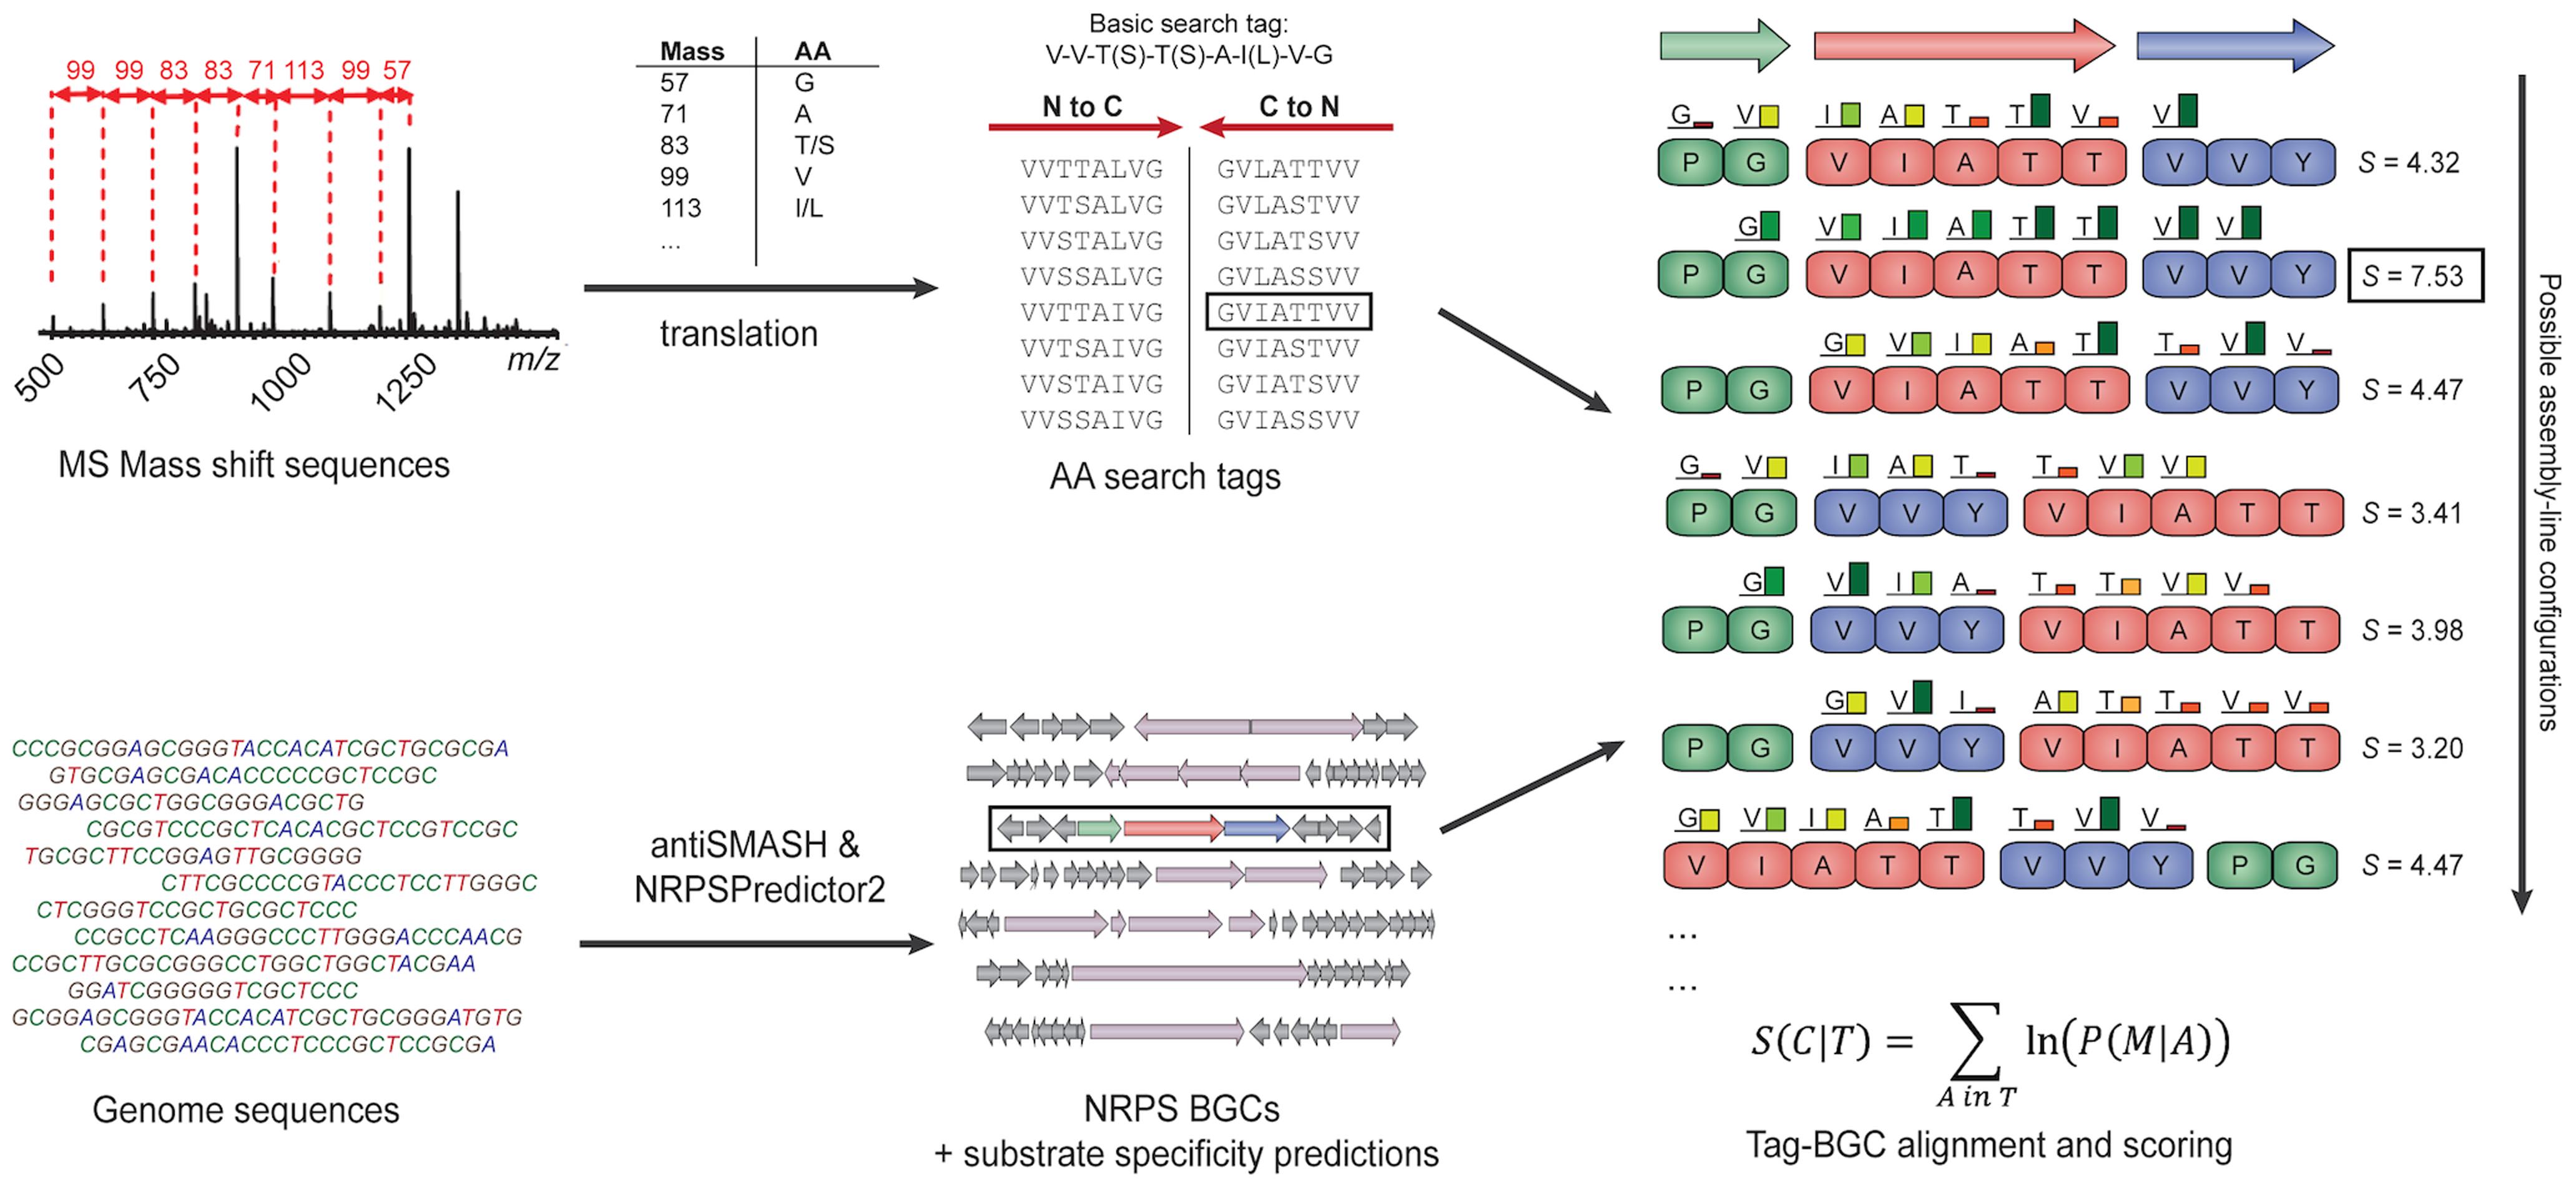
\includegraphics[width=1.25\linewidth]{images/nrp2path.png}}%

    \caption{An illustration of the NRP2Path algorithm. On the top is a mass spectrometry output being put through a mass translation table to produce
    a comprehensive list of potential sequence tags. On the bottom is BGC substrate specificity being extracted from raw sequence data by antiSMASH.
    These two sets of data are then used to compare every alignment of every sequence tag to every possible ordering of NRP blocks extracted from the 
    BGC. using the abbreviated scoring function shown below. Figure adapted from \cite{p2p}.
    }

    \label{fig:nrp2path}
\end{figure}

In order to compare a sequence tag to a BGC, NRP2Path uses its own scoring function loosely inspired by \textit{Bayes' Rule}. We omit the details of its derivation here for brevity's sake, but they are available in the original paper.

\scoreeqn

\(S(C|T)\) is the score of a gene cluster given the sequence tag. \(A\) is the amino acid making up part of a tag, and \(\mathbb{A}\) is the total amino acid alphabet being used. \(c\) and \(x\) are parameters that express the degree of confidence that final probability relies on substrate specificity rather than prior probability, and a pseudo-count to correct for small sample size, with default values \(c=1\) and \(x=0.01\), respectively. \(\eta\) is a regularisation term allowing for the exponential penalisation of repeated mismatches. \\

\(I_{A, M}\) is the average of two values calculated separately for the Stachelhaus Code and SVM predictions. The Code prediction is based on the closeness to the closest known NRPS module for NRPSPredictor2, whereas the SVM value is assigned between five evenly-spaced thresholds between 0 and 1 based on how closely the classes of the amino acid match (0 for no relation, 1 for exact match). \\

\(P(A)\) is the prior probability of \(A\), calculated like so:

\pa

where k is another pseudocount with k=1 and n(A) is the number of appearances within the NORINE database. \cit{norine}

Finally, the degree of matching between any gene sequence and mass spectrometry output is defined as the maximum of its scores across any alignment.

\subsection{RiPP2Path}

While RiPPQuest provides a method for the matching of BGCs to mass spectrometry readings in lanthipeptides, it does not cover all RiPPs. Following RiPPQuest, Pep2Path introduced RiPP2Path, a simple accessory tool for more broad matching of RiPPs. It functions by running a sliding window containing the sequence tag over every position of every translation frame in a gene sequence, computing the number of amino acid matches over the total length of the tag and then returning the highest scores.

Unlike RiPPQuest, this algorithm is naively targeted and processes a score for each gene subsequence, distinguishing them only by the score they receive. This does have penalties for accuracy where any identified sequence is more likely to have have appeared purely by random chance, especially in larger data, and costs more processing power inasmuch as it searches more, but it comes with the benefits of a very simple algorithm and is capable of applying the technology of peptidogenomics to all classes of RiPP, not just lanthipeptides.

%==================================================================================================================================
\chapter{Analysis/Requirements}

\section{Requirements}

For this project, the supervisor acted as a client, proposing the software for eventual integration into a larger codebase, and due to greater domain experience provided requirements implicitly as the project progressed. 

Firstly, we wanted a set of tools to implement the original Pep2Path functionality. This meant implementing NRP2Path and RiPP2Path. Secondly, the client had their own dataset for which the alignment comparison of NRP2Path might prove particularly cumbersome. This then meant being able to read the formats of the data available, and implement a simpler algorithm comparing the overlap between components. We also desired these implementations to be flexible with respect to future advances in bioinformatics, allowing the integration of custom scoring functions, as we outlined in the introduction. (\ref{motivation}) We implement these described algorithms both to solve this more proximal problem, and demonstrate the flexibility of our implementation.

The progam has to handle some very large search spaces, so efficiency is a concern. However, the client had a preliminary stage of screening for data reducing the data our implementation would have to process. Additionally, it would also be run on powerful hardware dedicated to processing very large bioinformatics data, so whilst it was necessary for our implementation to be efficient enough to terminate in reasonable time (and not, say, have unnecessary orders of complexity included within algorithms), the absolute highest degree of efficiency was not an aim for this project.

\textbf{<note to explain some of the other requirements below>}

We list functional requirements here using the MoSCoW method, and then non-functional requirements separately.

\subsection{Must Have}

\begin{itemize}

\item A mass spectrometry tool capable of converting mass/intensity readings to sequence tags.
\item Various small tools to be able to read in input data from standard file formats. Particularly, the ability to read the domain-standard antiSMASH-produced Genbank file formats.
\item A software base allowing the integration of custom scoring functions.
\item Implementation of a simpler BGC/mass-spectrometry comparison equivalent to taking the set intersection of the components in both, more suited to datasets with shorter sequence tags.
\item A full implementation of NRP2Path.
\item A suite of unit tests verifying the behaviour of the implementations of the various algorithms and improving future maintainability.
\end{itemize}

\subsection{Should Have}

\begin{itemize}
\item A full implementation of RiPP2Path.
\item The ability to run a 'many-to-many' comparison between BGC-predictions and mass spectrometry.
\item Replications of the original experimental results for Pep2Path (not necessarily exact, but on-target) to demonstrate functional correctness by practical test.
\item Integration with the client's codebase.
\end{itemize}

\subsection{Could Have}

\begin{itemize}
\item A simple CLI to run as a standalone.
\item An accessory visualisation tool to plot mass spectra with predicted sequence tags over them.
\item An adaptation of the RiPPQuest method to narrow down the translation around to just the region around the LANC-like domain for lanthipeptides.
\end{itemize}

\subsection{Won't Have}

\begin{itemize}
\item Implementations of novel scoring functions, such as one that takes advantage of antiSMASH 4's use of the SANDPUMA ensemble.
\item A full implementation of the RiPPQuest method for genome mining on lanthipeptides.
\end{itemize}

\subsection{Non-Functional Requirements}

\begin{itemize}
\item Should maintain strong separation of concerns and loose coupling, so components can be reused.
\item Platform-independence (portability).
\item Transparency of design.
\item A degree of efficiency - not a priority, but the program should avoid wasting time where possible.
\end{itemize}

%==================================================================================================================================
\chapter{Design}

\section{Software Structure}

\section{Algorithms}

\textbf{<note that throughout we use arbitrary user-provided mass-tables>}

\subsection{Mass Spectrum Dereplication}

The input to the \textit{de novo} mass spectrometry algorithm is a list of mass spectrometry readings, each with a mass value and an intensity value. First, we preprocess them to remove all low-intensity readings, according to some user-chosen threshold (perhaps 5\% of the maximum value), and sort them so that they are increasing order of mass. Then, we want to find gaps in the masses that correspond to the masses in some table of compounds (with some tolerance, either percentile or absolute). Then we want to find all sequences of masses where one mass begins on a peak as another ends, with no subsequences. This is just a matter of comparing masses then checking if they lie within some threshold.

We can formally model this problem as a \textbf{DAG} (Directed Acyclic Graph), a graph with a topological ordering - that is, each vertex is enumerated and vertices can only have edges to vertices with higher numbers. Furthermore, edges have a label, which is a list of all potential compounds that could be between the peaks the vertices represent, and these edges and their labels are unknown, but discoverable. In this model, vertices are individual mass spectrometry readings (mass and intensity), and edges are potential compounds from gaps between mass peaks. The problem of finding a sequence tag then corresponds to finding a path through this graph.

We partition this algorithm into two stages: edge discovery and path discovery. Edge discovery is the process of searching the raw numerical mass values of each peak for gaps corresponding to components in the mass table, in order to build the graph's edge set. Path discovery is then traversing the edges in the edge set in order to form a complete path - and therefore a sequence tag.

To perform edge discovery, we begin by allowing a value to be specified for a mass tolerance. This might be a static value measured in \textit{Da} (Unified Atomic Mass Unit or Dalton), a percentage applied to each mass in the mass table, or a percentage of the maximum mass in the spectra readings. We can then tranform each mass in the mass table into an interval \((mass - mass_tolerance, mass + mass_tolerance)\). Finally, we iterate through each reading, and subtract it from subsequent readings. If the result lies within the interval, then an edge exists between the peaks with a label corresponding to the compound which the interval belongs to. We repeat this for all values in the mass table in order to find all possible edges.

To perform path discovery

\begin{figure}
    \centering
    \makebox[\linewidth][c]{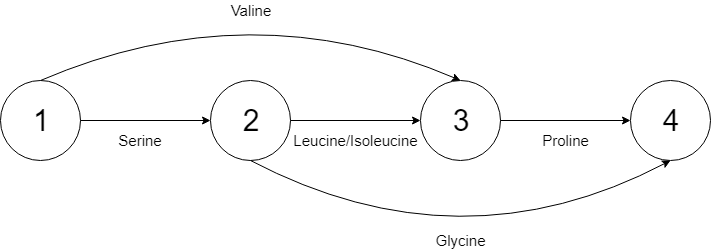
\includegraphics[width=1.0\linewidth]{images/peak_graph.png}}%

    \caption{An example illustration of some mass spectra peaks represented as a DAG, with arbitrarily chosen amino acid names for the edges. From this 	    graph there would be the tags (without subtags) Ser-Leu/Ile-Pro, Val-Pro, Ser-Gly.
    }

    \label{fig:peak_graph}
\end{figure}

\textbf{<note to mention optimisations, such as those in the mass spectrometry book>}

\subsection{NRPS2Path}
\textbf{<note to make it clear that we can check both directions of sequence tag in the NRPS algorithm by checking all module configurations against one sequence tag>}

\subsection{RiPP2Path}

This algorithm first reads in 

This algorithm bears some resemblance to brute-force string search, but whilst brute force string search searches for an exact match, this algorithm attempts to score every possible substring. We do this so as to provide as much information on the data as possible. For example, suppose that our search tag was one amino acid off, and we could not find it in the data. Then when attempting to find an exact match, we would only have a 'not found' result. But given this extra granularity, a near-total match would show up as the highest score found. 

\textbf{<note: should i move (parts of) this somewhere? the comparison to our method is useful...>}

However, as a result, this algorithm can't improve on the \(O(n^2)\) complexity of the most naive forms of brute-force string search (i.e. ones without early termination on the first mistmatch when aligning a substring with the query string), because improvements work by skipping some substrings. However, should we wish to search for exact matches, this is a solved problem with standard solutions, such as the linear-time Knuth-Morris-Pratt algorithm \cit{kmp}, the emprically performant Boyer-Moore algorithm \cit{boyer-moore} or algorithms such as hybrid KMP/BM algorithms. \cit{kmpbm} \cit{kmpbmtwo} String search algorithms such as these are also of more use in other areas of bioinformatics more generally as seen in the use of a hybrid KMP/Boyer-Moore in genome profiling in the recent PATSIM \cit{patsim} or an alternative exact string-searching algorithm TVSBS, \cit{tvsbs} designed specifically for biological sequence data. However, for most cases of exact string-matching GNU/Linux provides a standard, optimised implementation of Boyer-Moore as part of the \textit{grep} utility.

%==================================================================================================================================
\chapter{Implementation}

\section{Language Choice}

We chose to use Python for our implementation, as it is the \textit{lingua franca} of scientific computing. It offers highly expressive language constructs and useful libraries, such as itertools \cit{itools} offering many convenient ways to iterate through combinations, permutations and more, NumPy \cit{numpy} for high-speed numerical operations and BioPython \cit{biopy} for bioinformatics. All of these were used in the course of implementing our design. Additionally, a great volume of scientific software is already implemented in Python (indeed, the original Pep2Path is implemented using Python) and many scientists are familiar with Python already, making it easier to interface with the already extant body of work. Particularly, the client's codebase was implemented in Python, so this choice made for easier integration without the need for a language-spanning gateway. Other options like Julia \cit{julia} exist, but given their lack of maturity when compared to Python we elected not to explore these options.

%==================================================================================================================================
\chapter{Evaluation} 

%==================================================================================================================================
\chapter{Conclusion}    

%==================================================================================================================================
%
% 
%==================================================================================================================================
%  APPENDICES  

\begin{appendices}

\chapter{Appendices}

\end{appendices}

%==================================================================================================================================
%   BIBLIOGRAPHY   

% The bibliography style is abbrvnat
% The bibliography always appears last, after the appendices.

\bibliographystyle{abbrvnat}

\bibliography{l4proj}

\end{document}
